

\documentclass[10pt, conference, compsocconf]{IEEEtran}

\usepackage{cite}

\ifCLASSINFOpdf
\else
\fi

\usepackage{graphicx}
\usepackage{float}

\graphicspath{{figures/}}
\DeclareGraphicsExtensions{.pdf,.PDF,.png,.PNG}

\usepackage{balance}

\usepackage[draft]{hyperref}
\renewcommand{\sectionautorefname}{Section}
\renewcommand{\figureautorefname}{Fig.}

\usepackage{csquotes}
\usepackage{gensymb}

\hyphenation{op-tical net-works semi-conduc-tor}

\makeatletter
\g@addto@macro\@maketitle{
    \vspace{-1\baselineskip}
    \vspace{1.6\baselineskip}
    \begin{figure}[H]
        \setlength{\linewidth}{\textwidth}
        \setlength{\hsize}{\textwidth}
        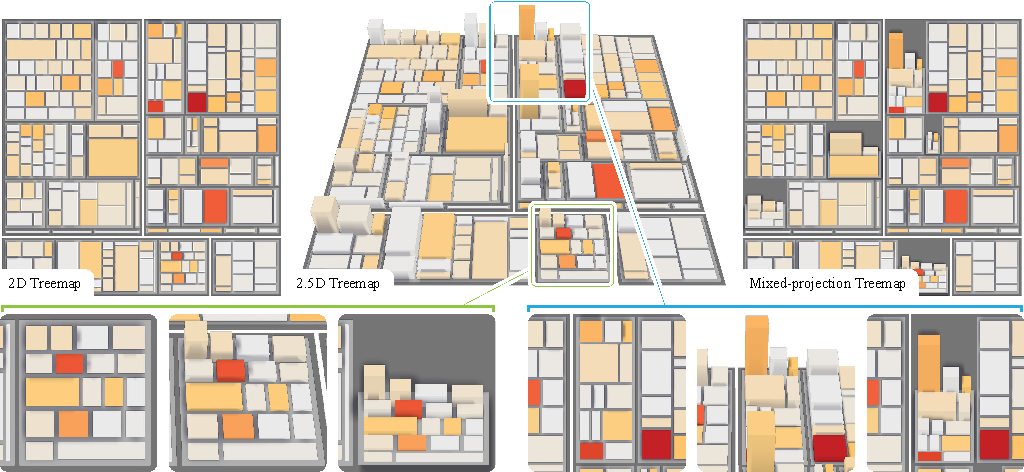
\includegraphics[width=\textwidth]{teaser}
        \caption{%
            2D treemap (left) and 2.5D treemap (center) depicting the same data using color and additional height mapping, respectively.
            A mixed-projection treemap (right), in contrast, reduces visual clutter and occlusion. At the same time, it exposes important correlations not accounted for in the 2D treemap.%
        }
        \label{fig:teaser}
        \label{fig:example-zoo}
    \end{figure}
}
\makeatother

\usepackage{xcolor}
\usepackage{eso-pic}
\AddToShipoutPictureFG{\AtPageLowerLeft{\put(\LenToUnit{0.5\paperwidth},\LenToUnit{6mm}){\makebox[0pt][c]{\fontsize{6.5}{8}\selectfont\color{gray}Author's revised version (2026-11-14). Version of record: \url{https://doi.org/10.1109/iV.2017.67}}}}}
\begin{document}
\title{Mixed-Projection Treemaps: A Novel Approach Mixing 2D and 2.5D Treemaps}

\author{%
    \IEEEauthorblockN{Daniel Limberger, Willy Scheibel, Matthias Trapp, and J\"urgen D\"ollner}
    \IEEEauthorblockA{%
        Hasso Plattner Institute---Faculty of Digital Engineering\\
        University of Potsdam, Germany\\
        \{daniel.limberger, willy.scheibel, matthias.trapp, juergen.doellner\}@hpi.de}
}

\maketitle

\begin{abstract}
This paper presents a novel technique for combining 2D and 2.5D treemaps using multi-perspective views to leverage the advantages of both treemap types.
It enables a new form of overview+detail visualization for tree-structured data and contributes new concepts for real-time rendering of and interaction with treemaps.
The technique operates by tilting the graphical elements representing inner nodes using affine transformations and animated state transitions.
We explain how to mix orthogonal and perspective projections within a single treemap.
Finally, we show application examples that benefit from the reduced interaction overhead.
\end{abstract}

\begin{IEEEkeywords}
Information Visualization; Overview+Detail; Treemaps; 2.5D Treemaps; Multi-perspective Views;
\end{IEEEkeywords}

\IEEEpeerreviewmaketitle


\section{Introduction}%
\label{sec:introduction}
\noindent
Treemaps represent a space-filling visualization technique that facilitates display and exploration of non-spatial, attributed, tree-structured data.
They map attributes to graphical elements, e.g., rectangles, that are recursively stacked within their parents' elements.
As one key advantage, 2D treemaps serve as a scalable visualization technique for tree-structured data~\cite{Fekete2002}.
They are applied in various research and industry applications to provide comprehensive and consistent means for communication and visual analytics~\cite{MacEachren1995} of non-spatial, massive, temporally and structurally evolving information such as file systems~\cite{Shneiderman1992} and software systems~\cite{Limberger2013}.
2.5D treemaps extend this concept by introducing height as another visual variable.
The 3D representation, however, leads to increased rendering effort, occlusion, and demands for advanced navigation techniques that counterbalance the advantages of 2.5D treemaps to a certain degree.

The expressiveness of 2D treemaps is limited compared to 2.5D treemaps taking advantage of the third dimension~\cite{Schulz2011}.
Apart from the height per graphical element, they also provide additional visual variables such as transparency, texture, shading, extended shape, as well as silhouette enhancement techniques~\cite{Limberger2016}.
Similar to 2D treemaps, 2.5D treemaps can be efficiently rendered~\cite{Trapp2013} and offer an additional dimension for information display.

2.5D treemaps are limited by a number of drawbacks~\cite{VanWijk2003,Schulz2011}, such as occlusion, underutilized screen-space, and perspective foreshortening---problems well known in the field of thematic 3D visualization~\cite{Elmqvist2008,Lorenz2008}.
Especially occlusion appears to have a \enquote{detrimental impact on discovering, accessing, and spatially relating embedded data}~\cite{Roehlig2016}.
In most applications though, occlusion is usually counterbalanced by a well-tuned \emph{map theme} (a task-centric specification of the attribute mapping to visual variables) and usually does not lead to a \enquote{significant loss of information}:
similar to the use of color, a meaningful use of height facilitates identification of relevant data by means of outlier perception, data range and distribution adjustments, as well as aggregation of irrelevant areas~\cite{Limberger2017}.
When applying these established operations, the resulting 2.5D treemaps consist mostly of flat cuboids.
However, when the input data is partially unknown or the task focuses on dynamic exploration, tuning the overall map theme might not be beneficial or appropriate at all and the visual complexity, e.g., by means of occlusion, can be hindering in the information gathering process.

This paper presents a novel visualization approach for treemaps that combines orthogonal and perspective projections within a single 2.5D treemap.
Thereby, it strengthens the applicability of treemaps by optimizing their compliance with the visual information seeking mantra \enquote{overview first, zoom and filter, then details-on-demand}~\cite{Shneiderman1996}.
For it, rendering and interaction techniques that enable 2D treemaps to get locally extended to 2.5D treemaps (\emph{mixed-projection treemaps}, \autoref{fig:teaser}) are introduced and the following contributions are made:
\begin{enumerate}
    \item A rendering technique that dynamically mixes different projections supporting seamless integration of 2.5D treemaps for regions of interest into 2D treemaps to facilitate communication of additional information using more visual variables.
    \item An interaction concept that enables users to control the projection by means of manual and automated tilting, either providing explicit control or using animated state transitions, respectively.
\end{enumerate}
We argue that interactive mixed-projection treemaps reduce the need for complex navigation metaphors typically associated with 2.5D treemaps and, further, feature traits common for \emph{focus+context} or \emph{overview+detail} metaphors, i.e., (1) the reduction of visual complexity for overview and context display and (2) the visualization of additional data in focus or detail areas. We demonstrate and discuss these aspects by means of application examples. %




\section{Related Work}
\label{sec:related}

\noindent
Treemaps are a common technique for space-restricted visualization of tree-structured data. The original algorithm presented by Shneiderman recursively splits parent nodes alternating in horizontal and vertical direction by their child nodes~\cite{Shneiderman1992}, resulting in a 2D layout.
By using specific shading~\cite{VanWijk1999}, margins or insets~\cite{Lue2008}, the treemap can depict topology as well.
Often used visual variables include size and color~\cite{Fekete2002} as well as texture~\cite{Holten2005}.

\paragraph{Treemap Layouts}

Besides treemap presentations, a basic layout algorithm has to be chosen according to the particular use cases.
For example, the choice of the layout algorithm influences the creation and preservation of a mental map for the user of the visualization~\cite{Misue1995}.
One major disadvantage of the Slice'n Dice algorithm is the creation of unfavorable aspect ratios of the node representations. Bruls et~al. as well as Bederson and Shneiderman counterbalance this problem using Squarified~\cite{Bruls1999} and Strip Treemap~\cite{Bederson2002} layouts.
Latest research focuses on the use of space-filling curves and further optimizes the trade-off between readability and stability~\cite{Tu2007,Tak2013}.
Since most of the treemap layout algorithms are designed for 2D presentation, they do not take possible occlusion within 2.5D treemaps into account.

\paragraph{2.5D Treemaps}

The first extension of 2D treemap algorithms to the third dimension is presented in the StepTree visualization system by Bladh et~al.~\cite{Bladh2004}. It extends the initial approach by stacking the graphical representations of subdirectories.
In a comparative study between the StepTree and its corresponding 2D treemap, users performed significantly better in tasks of interpreting the hierarchical structure while preserving performance in other interpretive and navigational tasks.
In addition to this approach, there exist a variety of modifications and extensions, e.g., 3D Polar Treemaps, Treecubes, or Collector's Box Treemaps~\cite{Schulz2011}.
In contrast to general 3D treemaps, most current 3D tree visualization techniques combine a 2D layout and extrude the graphical elements forming the third dimension.
Due to the restricted use of the third dimension, we refer to the term 2.5D treemaps.
An example of how to adaptively extend the nodes' shape in 2D treemaps by the third dimension was provided by Chaudhuri and Shen~\cite{Chaudhuri2009}.
Wettel and Lanza use 2.5D treemaps to create a metaphorical view on software system artifact hierarchies with CodeCities~\cite{Wettel2007} by mapping additional information to the height of leaf nodes.
Bohnet and D{\"o}llner mentioned the benefits of using realistic rendering effects (e.g., shadows) in 2.5D treemaps to support users in distinguishing individual elements~\cite{Bohnet2011}.

The increasing number of items in large hierarchies leads to perceptional questions about treemap visualizations, e.g., how much effect does the width of a node's border have on the ability to extract the hierarchical structure of the underlying data~\cite{Kong2010}.
With an increasing number of items, the need for focus+context as well as overview+detail techniques emerges~\cite{Hauser2006}.
Even though the visualization of a wide range of large hierarchical datasets (e.g., software systems, economy data) is frequently studied, the interaction techniques used in this field remain straightforward.
Apparent interaction techniques in 2.5D treemaps are the selection of inner nodes and leaves as well as the coloring/highlighting of nodes~\cite{Wettel2007}.
Sud et~al. present interactive rendering, navigation, and animation of dynamically changing 2D Voronoi Treemaps by using a GPGPU-based rendering technique~\cite{Sud2010}.

\paragraph{Mixed-perspective Visualization}

The choice for the type of projection for virtual 3D environments is often either an orthographic or perspective projection~\cite{Piringer2004}.
However, depending on the composition and the characteristics of the environment, mixed projections can provide effective communication of the content.
For virtual terrain and city model visualization, multi-perspective views with bent projections provide a near-field depiction of high detail and a context area of less detail~\cite{Pasewaldt2011,Roehlig2016}.
Before hardware-accelerated rendering techniques for mixed projections were developed~\cite{Lorenz2008}, these approaches were already applied by artists such as H.~C.~Berann~\cite{Berann1999}.


\section{Visualization}
\label{sec:visualization}
\noindent
This section (1) introduces a two-part tilt operator that uses a sequence of parameterized affine transformations, (2) describes a rendering that relies on a single geometry encoding and uses the exact same pipeline for both 2D and 2.5D nodes, and (3) specifies two interaction modes featuring manual and automated tilt control.

\subsection*{Node-local Tilt Operator}
\noindent
Given a 2D treemap, a tilt denotes the rotation of an inner node (and its children) that enables exploration of the height mapping using either an orthographic or perspective projection.
Any tilt comprises the following two node-local operations: a tilt transformation $\Lambda$ and a tilt projection $\Gamma$.

The tilt transformation shifts the node's rotation axis by $T_R$ using a relative offset $\tau\in\left[-1,+1\right]$, with $-1$ shifting to the node's bottom edge and $+1$ to its top edge.
It then rotates the node by the tilt angle $\alpha$ using $R$, and anchors the node by $T_A$ using a preferred relative location $\upsilon\in\left[-1,+1\right]$ (again, $-1$ at bottom and $+1$ at top, $0$ at center).
The complete, affine transformation (\autoref{fig:transformations}) is defined as
\begin{equation}
    \Lambda = \left[T_C\right] T_A T^{-1}_R R T_R.
\end{equation}
$T_C$ thereby denotes an optional translation that reduces occlusion introduced when using a perspective projection.
It can be easily derived using the virtual camera's eye position and, e.g., the node's vertical extent.
Also, we advise against deviating from $\tau=0$ (using perspective projection) since it either introduces more occlusion or reduces the node's size on display with $\tau>0$ and $\tau<0$ respectively.

The tilt projection basically mixes any two given projections $P_0$ and $P_1$ with respect to the node-local tilt angle and a global angular threshold $\beta$ and is defined as
\begin{equation}
    \Gamma = \left(1 - t\right) P_0 + t P_1,
\end{equation}
with $t = \alpha\beta^{-1}$, clamped to $\left[0,1\right]$.
If $P_1$ is a perspective projection, $P_0$ should be the respective orthographic projection, i.e., it should cover the exact same treemap region.

Even though both transformation and projection are applied per-node and can be at different states at any time for any node, they are restricted to global parameters for $\beta$, $\tau$, and $\upsilon$ provided by the map theme.
For a seamless tilt transition only $\alpha$ has to be increased, starting at $\alpha = 0$ for no transition up to the desired, final tilt angle.
\begin{figure}[t!]
    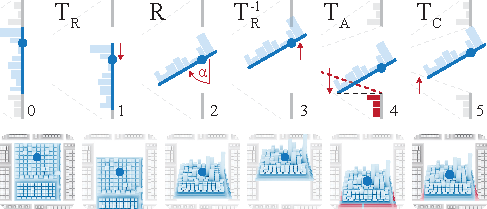
\includegraphics[width=\linewidth]{transformations}
    \caption{This illustration describes a tilt transformation $\Lambda$ of an inner node $n$ with perspective projection applied: $n$ is (1) translated by $T_R$ for (2) rotation by $R$ with $\alpha=60\degree$ at the local tilt offset $\tau=0.5$. After (3) translating $n$ ($T^{-1}_R$) it is (4) moved to the bottom anchor by $T_A$ with $\upsilon=-1$ and, finally, (5) shifted up again by $T_C$ in order to reduce the occlusion caused by the perspective projection. Step (5) is only required when using orthogonal projection.}
    \label{fig:transformations}
\end{figure}

\subsection*{Rendering}
\noindent
For the interactive use of mixed-projection treemaps a real-time rendering based on attributed vertex clouds \cite{Scheibel2017} is used.
It allows for efficient GPU encoding of hierarchical information and facilitates interactive, dynamic attribute mapping, and on-the-fly, attribute-based geometry instantiation.
The use of the node-local tilt operator allows us to rely solely on a 2.5D GPU encoding for simultaneously rendering some nodes in 2D and others in 2.5D (either orthographic or perspective).
This means that the height mapping is always enabled, but not noticeable on nodes that are not tilted.
Furthermore, the same rendering pipeline can be applied to all nodes.
It ultimately enables a seamless transition between 2D and 2.5D as well as orthographic and perspective projections, especially since the results of screen-space effects remain consistent w.r.t. shading, local ambient occlusion, shadows, contouring etc.

\subsection*{Interaction}
\noindent
Navigation in 2.5D treemaps can be implemented by means of a landscape metaphor or world-in-hand metaphor.
In the case of mixed-projection treemaps, however, a simple zoom and pan metaphor is sufficient for navigating the treemap.
Based on the parameterization introduced previously, a user can interact directly with treemap nodes based on direct manipulation metaphors.
For it, we suggest two similar tilt modes: \emph{manual tilt} and
\emph{automated tilt}.
A manual tilt enables the user to increase and decrease the tilt angle of any node seamlessly (e.g., via click/touch to an inner node and vertical drag down).
An automated tilt enables the user to invoke a preset tilt angle or un-tilt any node by a single input event (e.g., click/touch to an inner node).
To avoid abrupt tilt angle changes, an animated transition with arbitrary easing can be applied.
Due to the simplicity of both tilt interactions, additional interactions (e.g., filtering) can be integrated more easily.
Both modes can also be combined by applying some type of mode switch.
Keep in mind though that the tilt is not designed for nested application.


\section{Results}
\label{sec:results}

\noindent
When using mixed-projection treemaps to visualize tree-structured data, the designated use case follows a multi-step process.
First, the user gains overview using the 2D top view on the treemap rendered with orthographic projection.
For all areas-of-interest, the user can select the inner nodes.
Those selected nodes are then tilted into a 2.5D presentation with additional visual variables.
The prototypical implementation is an extension to a 2.5D treemap visualization system by means of
(1) the management of selected inner nodes for the detail view,
(2) computing the nodes' geometry tilting,
(3) efficient image synthesis using an attributed vertex cloud of axis-aligned cuboids where
(4) the tilt is applied during geometry instantiation~\cite{Scheibel2017}.

\subsection*{Application Examples}

\noindent
Mixed-projection treemaps support in getting an overview over a dataset first and finding relevant nodes afterwards by enabling the third dimension on-demand.
As examples of real-world tree-structured datasets we chose a population count dataset and a software system dataset.

\paragraph{Population Count Dataset}
The first dataset is the population count of the zoo in Munich from 2014 (\autoref{fig:example-zoo}).
The dataset contains 247~nodes whereby each node represents one species.
The footprint size of a visual item refers to the population count of a species, the color refers to the extinction threat index, and the number of born animals in the last year is mapped to the height.
This map theme facilitates the detection of recovering species.

\paragraph{Software System Dataset}
The second dataset represents an analysis of the open-source project POCO\footnote{GitHub project available at \url{github.com/pocoproject/poco}; Analysis of revision from March 24 in 2009.} (\autoref{fig:example-poco}).
The dataset contains 5775~nodes.
Each node represents one source code file.
The number of real-lines-of-code is mapped to the footprint size, the color refers to cyclomatic complexity, and the average nesting level of a source code file is mapped to the height.
This map theme is primarily used to detect source code files with disproportional nesting level in comparison to the implemented business logic.

\subsection*{Discussion}
\noindent
While the process is set, the actual depiction of selected nodes is subject to discussion.
There are different approaches for setting the tilt anchor, angle, and additional occlusion-reducing rotation.
To support users in maintaining their mental map, animated transition and different types of perspectives can be applied.

\paragraph{Perspective vs. Orthographic Projection}
Due to perspective foreshortening in a perspective view (the default for virtual 3D environments), objects that are far form the virtual camera away are rendered smaller than closer ones. Alternatively, in an orthographic view, all objects appear at same scale. Since the user preference of projection may differ, both options are supported: (1) perspective projections provide additional information about depth and are often easier to interpret, and (2) orthographic projections facilitate comparison of nodes w.r.t. height and area.
Further, an orthographic projection renders no occlusion to neighboring nodes in the overview.

\paragraph{Tilt Anchor}
After tilting the inner nodes, the inclination introduces unused screen space.
This may be partially covered by higher nodes but the overall impression remains and even supports the identification of these nodes as tilted (and thus, conveying height information).
To exploit this space further, the tilted node can be shifted within the original bounding rectangle (\autoref{fig:tilt-anchor}).
\begin{figure}[h!]
    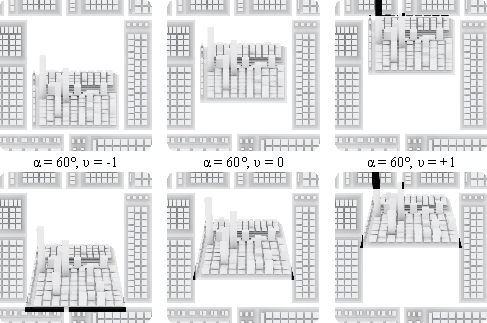
\includegraphics[width=\linewidth]{results-anchor}
    \caption{Orthogonal (top row) and perspective (bottom row) projections anchored at different locations, all tilted by 60° (overdraw colored black).}
    \label{fig:tilt-anchor}
\end{figure}

\noindent
During experiments we made the following observation: the lower alignment seems to be most beneficial as the risk of occluding nearby nodes is minimized (compare to the right pictogram with top alignment; overdraw is colored black) and there is still sufficient space for possible additional information display (as opposed to the center alignment with justified whitespace, compare center pictogram).

\paragraph{Tilt Angle}
The effective tilt angle is subject to inner-node complexity and height-value distribution. Although angles between 0\degree{} and 90\degree{} are possible, a tilt degree of $\alpha= 0\degree$ results in no additional height information and a tilt of $\alpha = 90\degree$yields high occlusion (\autoref{fig:tilt-angle}).
\begin{figure}[h!]
    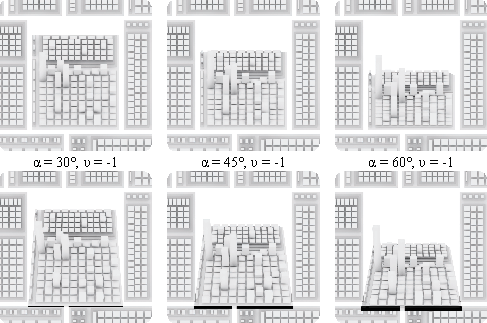
\includegraphics[width=\linewidth]{results-30-45-60}
    \caption{Orthogonal (top row) and perspective (bottom row) projections at different tilt angles, all anchored at the bottom (overdraw colored black).}
    \label{fig:tilt-angle}
\end{figure}
We found tilt angles between $30\degree$ and $60\degree$ to be reasonable supportive.
We also found that a slightly different shading of the cuboids' lateral surfaces servers as additional tilt cue.

\paragraph{Tilt Transitions}
Even though the mixed-projection treemap is designed for static display, the use of manual or animated transitions can help a user to maintain its mental map during the state change from overview to detailed depiction of an inner node and is highly suggested.

\begin{figure}[b!]
    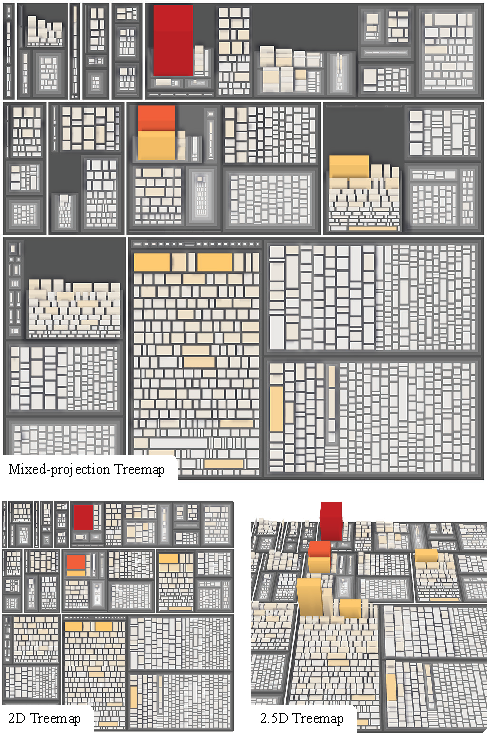
\includegraphics[width=\linewidth]{results-poco}
    \caption{A 2D treemap, 2.5D treemap, and a mixed-projection treemap (with various nodes tilted), all three of which depict the same POCO software system.}
    \label{fig:example-poco}
\end{figure}


\section{Conclusion and Future Work}
\label{sec:conclusions}

\noindent
This paper presents how to combine 2D and 2.5D treemaps.
The concept is based on in-situ mixed projections, i.e., the dynamic adjustment of and interpolation between orthographic and perspective projections of components of a single treemap based on regions of interest, which can be interactively selected by a user.
The combination strengthens the particular advantages of each projection technique: the overview and simple interaction with tree-structured data using 2D treemaps and the advanced capabilities of presenting additional data attributes using 2.5D treemaps.
To some extent it counterbalances the limitations inherent to 2.5D treemaps, e.g., occlusion and perspective-foreshortening.
It also simplifies the user interactions required for 2.5D treemaps.
Preliminary results obtained by using our prototypical implementation indicate a simplified treemap exploration and effective comparison of additional data mapped to height.
For future work we plan to take into account the available screen space for display of additional information using data charts such as histograms.


\balance

\section*{Acknowledgment}
\noindent
This work was funded by the Federal Ministry of Education and Research (BMBF), Germany, within the InnoProfile Transfer research group \enquote{4DnD-Vis} (\href{www.4dndvis.de}{www.4dndvis.de}).

\bibliographystyle{IEEEtran}
\bibliography{IEEEabrv,references}

\end{document}

